\documentclass{article}
\usepackage{graphicx}
\usepackage{multicol} % use to multiple column in itemize
\usepackage{float}
\usepackage{setspace}
\setlength{\parskip}{0.5em}

\begin{document}

\title{Introduction to Machine Learning}
\author{Cong Cuong PHAM}

\maketitle

\begin{abstract}
This document introduces some fundamental notions of Machine Learning.
\end{abstract}

\section{Introduction}
\subsection{What is Machine Learning?}
\begin{itemize}
	\item ML is a method of data analysis that automates analytical model building.
	\item Using algorithms that iteratively learn from data, ML allows computers to find hidden insights without being explicitly programmed where to look.
\end{itemize}

\subsection{What is Machine Learning used for?}
\begin{multicols}{2}
	\begin{itemize}
		\item Fraud detection.
		\item Web search results.
		\item Real-time ads on web pages.
		\item Credit scoring and next-best offers.
		\item Prediction of equipment models.
		\item New pricing models.
		\item Network intrusion detection.
		\item Recommendation Engines.
		\item Customer Segmentation.
		\item Text Sentiment Analysis.
		\item Predicting Customer Churn.
		\item Pattern and image recognition.
		\item Email Spam filtering.
		\item Financial Modeling.
	\end{itemize}
\end{multicols}

\subsection{ML Process}
\begin{figure}[H]
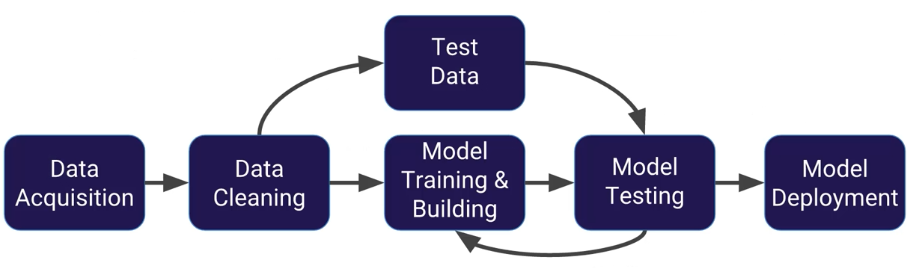
\includegraphics[width=\linewidth]{pic/ML-process.png}
\caption{Machine Learning Process}
\centering
\end{figure}

\subsection{Types of Machine Learning Algorithms}
\begin{itemize}
	\item Supervised Learning.
	\item Unsupervised Learning.
	\item Reinforcement Learning.
\end{itemize}

\subsubsection{Supervised Learning}
\par Is provided with a set of labeled data and is trying to predict a label based of known features.

\par The learning algorithm receives a set of inputs along with the corresponding correct outputs, and the algorithm learns by comparing its actual output with correct outputs to find errors. It then modifies the model accordingly.

\par Though methods like classification, regression, prediction and gradient boosting, supervised learning uses patterns to predict the values of the label on additional unlabeled data.

\par Supervised learning is commonly used in applications where historical data predicts likely future events.

\par Example: Anticipate when credit card transactions are likely to be fraudulent or which insurance customer is likely to file a claim; Predict the price of house based on different features for house for which we have historical price data.

\subsubsection{Unsupervised Learning}
\par Is used against data that has no historical labels. The system is not told the ``right answer''. The algorithm must figure out what is being shown.

\par The gold is to explore the data and find some structure within. It can find the main attributes that separate customer segments from each other.

\par Popular techniques include self-organizing maps, nearest-neighbor mapping, k-means clustering and singular value decomposition.

\par Example: Segment text topics, recommend items and identify data outliers.

\subsubsection{Reinforcement Learning}
\par Is often used for robotics, gaming and navigation. With reinforcement learning, the algorithm discovers through trial and error which actions yield the greatest rewards.

\par This type of learning has three primary components: the agent (the learner or decision maker), the environment (everything the agent interacts with) and actions (what the agent can do). The objective is for the agent to choose actions that maximize the expected reward over a given amount of time. The agent will reach the goal much faster by following a good policy.
\par The goal in reinforcement learning is to learn the best policy.
\end{document}

